\documentclass[english]{article}
\usepackage[T1]{fontenc}
\usepackage[latin9]{inputenc}
\usepackage{amstext}
\usepackage{babel,color}
\usepackage{amsmath}
\usepackage{amssymb}
\usepackage{geometry}
\usepackage{graphicx}
\usepackage{epstopdf}
\geometry{letterpaper,tmargin=1in,bmargin=1in,lmargin=1in,rmargin=1in}
%\usepackage[parfill]{parskip}    % Activate to begin paragraphs with an empty line rather than an indent
\parskip = 0.03in

\newtheorem{theorem}{Theorem}
\title{Gaussian Setting Detection Proofs}
\input my_header.tex

\begin{document}

\maketitle

\section*{Vector Case with Estimated Mean}

We consider the following binary classification problem:

\begin{equation}
y=\left\{
\begin{aligned}
&\mu_0+z
&& y\in H_0\\
&\mu_1+z
&& y\in H_1\\
\end{aligned}\right.
\end{equation}

where $z\in\reals^n, z\sim\mathcal{N}(0,I)$. We assume that $\mu_0,\mu_1\in\reals^n$ are unknown but we have estimates $\hat{\mu}_0, \hat{\mu}_1$ which were estimated from the data. We assume that $f(\mu_0|\hat{\mu}_0)\sim\mathcal{N}(0,\sigma_0^2I)$ and $f(\mu_1|\hat{\mu}_1)\sim\mathcal{N}(1,\sigma_1^2I)$

Let $\tilde{\mu}_0=\mu_0|\hat{\mu}_0$ and $\tilde{\mu}_1=\mu_1|\hat{\mu}_1$ so our new classification problem becomes

\begin{equation}\label{eq:y dist}
y=\left\{
\begin{aligned}
&\tilde{\mu}_0+z
&& y\in H_0\\
&\tilde{\mu}_1+z
&& y\in H_1\\
\end{aligned}\right.
\end{equation}

where $z\sim\mathcal{N}(0,I), \tilde{\mu}_0\sim\mathcal{N}(0,\sigma_0^2I),\tilde{\mu}_1\sim\mathcal{N}(0,\sigma_1^2I)$.

Under $H_0$, $y\sim\mathcal{N}(0,(1+\sigma_0^2)I)$ and under $H_1$, $y\sim\mathcal{N}(0,(1+\sigma_1^2)I)$. Our LRT is

\begin{equation}
\begin{aligned}
&\Lambda(y)=\frac{f_1(y)}{f_0(y)}
&&=
&&&\frac{(2\pi(1+\sigma_1^2))^{-n/2}\exp\{\frac{-1}{2(1+\sigma_1^2)}y^Ty\}}{(2\pi(1+\sigma_0^2))^{-1/2}\exp\{\frac{-1}{2(1+\sigma_0^2)}y^Ty\}}\\
&&&=
&&&\left(\frac{1+\sigma_0^2}{1+\sigma_1^2}\right) ^{n/2}\exp\left\{\frac{-y^Ty}{2}\left(\frac{1}{1+\sigma_1^2}-\frac{1}{1+\sigma_0^2}\right)\right\}\\
&&&=
&&&\left(\frac{1+\sigma_0^2}{1+\sigma_1^2}\right) ^{n/2}\exp\left\{\frac{-y^Ty}{2}\left(\frac{\sigma_0^2-\sigma_1^2}{(1+\sigma_1^2)(1+\sigma_0^2)}\right)\right\}\\
\end{aligned}
\end{equation}

Where our decision is

\begin{equation}
\begin{aligned}
&\text{Declare } H_0 \text{ if}
&& \Lambda(y) < \eta\\
& \text{Declare } H_1 \text{ if}
&& \Lambda(y) > \eta
\end{aligned}
\end{equation}

Defining

\begin{equation}
\hat{\Lambda}(y)=\frac{y^Ty}{2}\left(\frac{\sigma^2_1-\sigma^2_1}{(1+\sigma_1^2)(1+\sigma_0^2)}\right)
\end{equation}

our decision becomes

\begin{equation}
\begin{aligned}
&\text{Declare } H_0 \text{ if}
&& \hat{\Lambda}(y) < \ln\left(\eta\left(\frac{1+\sigma_1^2}{1+\sigma_0^2}\right)^{n/2}\right)\\
& \text{Declare } H_1 \text{ if}
&& \hat{\Lambda}(y) > \ln\left(\eta\left(\frac{1+\sigma_1^2}{1+\sigma_0^2}\right)^{n/2}\right)
\end{aligned}
\end{equation}

We assume that $\sigma_1^2>\sigma_0^2$. If this is not the case, we may simply reverse the roles of $H_0,H_1$. Defining

\begin{equation}
\gamma = \frac{2(1+\sigma_1^2)(1+\sigma_0^2)}{\sigma_1^2-\sigma_0^2}\left(\ln(\eta) +(n/2)\ln\left(\frac{1+\sigma_1^2}{1+\sigma_0^2}\right)\right)
\end{equation}

Our decision becomes

\begin{equation}
\begin{aligned}
&\text{Declare } H_0 \text{ if}
&& y^Ty < \gamma\\
& \text{Declare } H_1 \text{ if}
&& y^Ty > \gamma\\
\end{aligned}
\end{equation}

In the case where each class is equally likely $(\eta=1)$, this reduces to

\begin{equation}
\hat{\gamma} = \frac{n(1+\sigma_1^2)(1+\sigma_0^2)}{\sigma_1^2-\sigma_0^2}\ln\left(\frac{1+\sigma_1^2}{1+\sigma_0^2}\right)
\end{equation}

\begin{equation}
\begin{aligned}
&\text{Declare } H_0 \text{ if}
&& y^Ty < \hat{\gamma}\\
& \text{Declare } H_1 \text{ if}
&& y^Ty > \hat{\gamma}\\
\end{aligned}
\end{equation}

Define our test statistic as $\tau=y^Ty$. We seek the distribution of $\tau$ under $H_0$. Now $\tau=\sum_{i=1}^ny_i^2$. Under $H_0$, $y_i\sim\mathcal{N}(0,\sigma_0^2)$. Therefore under $H_0$,

\begin{equation}
\frac{\tau}{\sigma_0^2}=\sum_{i=1}^n\left(\frac{y_i}{\sigma_0}\right)^2
\end{equation}

which is a sum of standard normal Gaussians. Therefore, $\frac{\tau}{\sigma_0^2}\sim\chi_n^2$. Similarly, under $H_1, \frac{\tau}{\sigma_1^2}\sim\chi_n^2$. We can now set $\gamma$ to achieve a false alarm right $\alpha$.

\begin{equation}
P_F=P(\tau>\gamma | \text{under} H_0) = P(\frac{\tau}{\sigma_0^2}>\frac{\gamma}{\sigma_0^2} | \text{under} H_0) = Q_{\chi_n^2}(\frac{\gamma}{\sigma_0^2})
\end{equation}

We can then solve for $\gamma$

\begin{equation}\label{eq:gamma}
\gamma = \sigma_0^2Q^{-1}_{\chi_n^2}\left(P_F\right)
\end{equation}

which we can then uses to develop a relationship between $P_F$ and $P_D$

\begin{equation}
P_D=P(\tau>\gamma | \text{under} H_1) = P(\frac{\tau}{\sigma_1^2}>\frac{\gamma}{\sigma_1^2} | \text{under} H_1) = Q_{\chi_n^2}\left(\frac{\gamma}{\sigma_1^2}\right)
\end{equation}

Substituting our expression for $\gamma$ in (\ref{eq:gamma}) we have

\begin{equation}
P_D=Q_{\chi_n^2}\left(\frac{\sigma_0^2}{\sigma_1^2}Q^{-1}_{\chi_n^2}\left(P_F\right)\right)
\end{equation}

\section*{Processed Observation with Estimated Mean}

We now consider the case where we are not given $y$ explicitly but instead a processed version of it. That is

\begin{equation}
t=\left\{
\begin{aligned}
&U_0^Ty
&& t\in H_0\\
&U_1^Ty
&& t\in H_1\\
\end{aligned}\right.
\end{equation}

where $U_1, U_2\in\reals^{n\times p}$ are known have orthonomal columns and $t\in\reals^p$. We therefore have the detection problem

\begin{equation}
t=\left\{
\begin{aligned}
&U_0^T\mu_0 + U_0^Tz
&& t\in H_0\\
&U_1^T\mu_1 + U_1^Tz
&& t\in H_1\\
\end{aligned}\right.
\end{equation}

where $z\in\reals^n, z\sim\mathcal{N}(0,I)$. We assume that $\mu_0,\mu_1\in\reals^n$ are unknown but we have estimates $\hat{\mu}_0, \hat{\mu}_1$ which were estimated from the data. We assume that $f(\mu_0|\hat{\mu}_0)\sim\mathcal{N}(0,\sigma_0^2I)$ and $f(\mu_1|\hat{\mu}_1)\sim\mathcal{N}(1,\sigma_1^2I)$. As $U_0,U_1$ have orthonormal columns, $U_0z, U_1z$ are both $\mathcal{N}(0,I_{p\times p})$. Let $\tilde{z}\sim\mathcal{N}(0,I_{p\times p})$. Let $\tilde{\mu}_0=\mu_0|\hat{\mu}_0$ and $\tilde{\mu}_1=\mu_1|\hat{\mu}_1$ so our new classification problem becomes

\begin{equation}
t=\left\{
\begin{aligned}
&U_0^T\tilde{\mu}_0 + \tilde{z}
&& t\in H_0\\
&U_1^T\tilde{\mu}_1 + \tilde{z}
&& t\in H_1\\
\end{aligned}\right.
\end{equation}

Under $H_0, t\sim\mathcal{N}(0,\sigma_0^2I_{p\times p})$ and under $H_1, t\sim\mathcal{N}(0,\sigma_1^2I_{p\times p})$

Similar to the previous section, this yields the detector

\begin{equation}
\begin{aligned}
&\text{Declare } H_0 \text{ if}
&& t^Tt < \frac{2(1+\sigma_1^2)(1+\sigma_0^2)}{\sigma_1^2-\sigma_0^2}\left(\ln(\eta) +(p/2)\ln\left(\frac{1+\sigma_1^2}{1+\sigma_0^2}\right)\right)\\
& \text{Declare } H_1 \text{ if}
&& t^Tt > \frac{2(1+\sigma_1^2)(1+\sigma_0^2)}{\sigma_1^2-\sigma_0^2}\left(\ln(\eta) +(p/2)\ln\left(\frac{1+\sigma_1^2}{1+\sigma_0^2}\right)\right)\\
\end{aligned}
\end{equation}

Using a similar analysis to the previous section, we can establish a relationship between $P_D$ and $P_F$ using the distribution of our test statistic $t^Tt$ and arrive at

\begin{equation}
P_D=Q_{\chi_p^2}\left(\frac{\sigma_0^2}{\sigma_1^2}Q^{-1}_{\chi_p^2}\left(P_F\right)\right)
\end{equation}

with the only difference being the degrees of freedom of our chi-square distribution.

\section*{Numerical Results}

We plot the theoretical ROC curves derived in each of the previous two sections. The only difference between the two being the dimension of the test statistic which results in different degrees of freedom in the resulting chi-square distribution. We can see that when we reduce the dimension of our problem, we push the ROC curve to the bottom right which is evidence of a worse detector. The larger the ratio of $n/p$ results in a larger decrease in detection power. The larger the ratio of $\sigma_1^2/\sigma_0^2$ results in overall better detectors (for both detectors). This intuitively makes sense as our observed points will be clustered more sparsely and easier to differentiate.

\begin{figure}
\centering
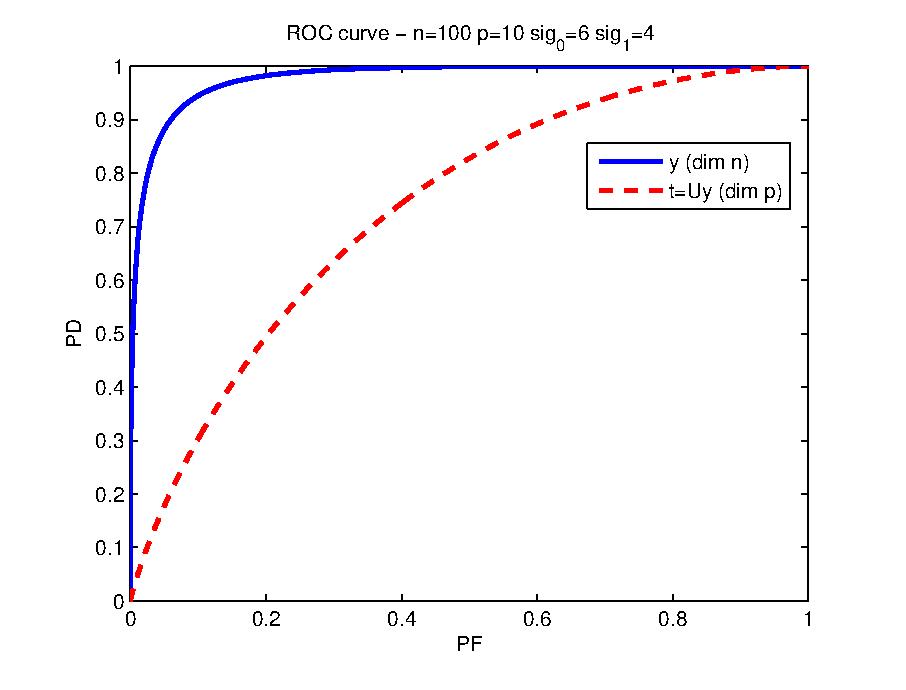
\includegraphics[width=5in]{roc_curve}
\end{figure}

\section*{Stochastic Model}

We begin with the following stochastic binary classification problem:

\begin{equation}
y=\left\{
\begin{aligned}
&U_0x+z
&& y\in H_0\\
&U_1x+z
&& y\in H_1\\
\end{aligned}\right.
\end{equation}

where $z\in\reals^n, z\sim\mathcal{N}(0,I)$. We assume that $U_0,U_1\in\reals^{n\times p}$ are known and have orthonormal columns. We assume $x\in\reals^p$ and $f(x|H_0)\sim\mathcal{N}(0,\Sigma_0),~f(x|H_1)\sim\mathcal{N}(0,\Sigma_1)$. An extension to (\ref{eq:y dist}), shows that under $H_0$, $y\sim\mathcal{N}(0, U_0\Sigma_0U_0^T + I)$ and under $H_1$, $y\sim\mathcal{N}(0, U_1\Sigma_1U_1^T + I)$

We now consider the case where we are not given $y$ explicitly but instead a processed version of it. That is

\begin{equation}
t=\left\{
\begin{aligned}
&U_0^Ty
&& t\in H_0\\
&U_1^Ty
&& t\in H_1\\
\end{aligned}\right.
\end{equation}

By properties of Gaussian random variables, under $H_0$, $y\sim\mathcal{N}(0, U_0^TU_0\Sigma_0U_0^TU_0 + U_0^TU_0)$ and under $H_1$, $y\sim\mathcal{N}(0, U_1^TU_1\Sigma_1U_1^TU_1 + U_1^TU_1)$. Recalling that $U_0,U_1$ have orthonormal columns, we have that under $H_0$, $t\sim\mathcal{N}(0,I+\Sigma_0)$ and under $H_1$, $t\sim\mathcal{N}(0,I+\Sigma_1)$. Our LRT is

\begin{equation}
\begin{aligned}
&\Lambda(t) = \frac{f_1(t)}{f_0(t)}
&& =
&&&\frac{(2\pi)^{-p/2}|I+\Sigma_0|^{-1/2}\exp\{-\frac{1}{2}t^T(I+\Sigma_0)^{-1}t\}}{(2\pi)^{-p/2}|I+\Sigma_1|^{-1/2}\exp\{-\frac{1}{2}t^T(I+\Sigma_1)^{-1}t\}}\\
&&& =
&&& \left(\frac{|I+\Sigma_1|}{|I+\Sigma_0|}\right)^{1/2}\exp\{-\frac{1}{2}t^T\left[\left(I+\Sigma_0\right)^{-1}-\left(I+\Sigma_1\right)^{-1}\right]t\}\\
\end{aligned}
\end{equation}

where our decision is

\begin{equation}
\begin{aligned}
&\text{Declare } H_0 \text{ if}
&& \Lambda(t) < \eta\\
& \text{Declare } H_1 \text{ if}
&& \Lambda(t) > \eta
\end{aligned}
\end{equation}

Since $\Sigma_0,\Sigma_1$ are valid covariance matrices, $|I+\Sigma_0|\succeq0,~|I+\Sigma_1|\succeq0$. Therefore, if we define

\begin{equation}
\tilde{\Lambda}(t) = t^T\left[\left(I+\Sigma_0\right)^{-1}-\left(I+\Sigma_1\right)^{-1}\right]t
\end{equation}

our decision becomes

\begin{equation}
\begin{aligned}
&\text{Declare } H_0 \text{ if}
&& \tilde{\Lambda}(t) < 2\ln(\eta)+\ln\left(\frac{|I+\Sigma_0|}{|I+\Sigma_1|}\right)\\
& \text{Declare } H_1 \text{ if}
&& \tilde{\Lambda}(t) > 2\ln(\eta)+\ln\left(\frac{|I+\Sigma_0|}{|I+\Sigma_1|}\right)
\end{aligned}
\end{equation}

Defining $A=\left(I+\Sigma_0\right)^{-1}-\left(I+\Sigma_1\right)^{-1}$, our statistic is $\tau=t^TAt$.

There is no closed form solution for the distribution of $\tau$ unless $A$ is diagonal, which results from $\Sigma_1,\Sigma_0$ also being diagonal and some other cases as well.

\section*{Stochastic setting Estimated Subspaces}

We again consider

\begin{equation}
y=\left\{
\begin{aligned}
&U_0x+z
&& y\in H_0\\
&U_1x+z
&& y\in H_1\\
\end{aligned}\right.
\end{equation}

where $z\in\reals^n, z\sim\mathcal{N}(0,I)$. We assume that $U_0,U_1\in\reals^{n\times p}$ are unknown and have orthonormal columns. We assume $x\in\reals^p$ and $f(x|H_0)\sim\mathcal{N}(0,\Sigma_0),~f(x|H_1)\sim\mathcal{N}(0,\Sigma_1)$. An extension to (\ref{eq:y dist}), shows that under $H_0$, $y\sim\mathcal{N}(0, U_0\Sigma_0U_0^T + I)$ and under $H_1$, $y\sim\mathcal{N}(0, U_1\Sigma_1U_1^T + I)$

We now consider the case where we are not given $y$ explicitly but instead a processed version of it, using estimates $\hat{U}_0,\hat{U}_1$ of our underlying subspaces, $U_0, U_1$. $U_0,U_1,\hat{U}_0,\hat{U}_1$ all have orthonormal columns. We distinguish between our testing and training data. Our estimates $\hat{U}_0,\hat{U}_1$ are formed from our training data:

\begin{equation}
y_{\text{train}}=\left\{
\begin{aligned}
&U_0x_{\text{train}}+z_{\text{train}}
&& y_{\text{train}}\in H_0\\
&U_1x_{\text{train}}+z_{\text{train}}
&& y_{\text{train}}\in H_1\\
\end{aligned}\right.
\end{equation}

where $z_{\text{train}}\in\reals^n, z\sim\mathcal{N}(0,I)$. We assume that $U_0,U_1\in\reals^{n\times p}$ are unknown and have orthonormal columns. We assume $x_{\text{train}}\in\reals^p$ and $f(x_{\text{train}}|H_0)\sim\mathcal{N}(0,\Sigma_{\text{train}0}), ~f(x_{\text{train}}|H_1)\sim\mathcal{N}(0,\Sigma_{\text{train}1})$. Our estimates are formed from the leftmost left singular vectors of the SVD composition of the matrix formed by stacking the labeled training data in columns.

Our problem becomes

\begin{equation}
t=\left\{
\begin{aligned}
&\hat{U}_0^Ty
&& t\in H_0\\
&\hat{U}_1^Ty
&& t\in H_1\\
\end{aligned}\right.
\end{equation}

By properties of Gaussian random variables, under $H_0$, $y\sim\mathcal{N}(0, \hat{U}_0^TU_0\Sigma_0U_0^T\hat{U}_0 + \hat{U}_0^T\hat{U}_0)$ and under $H_1$, $y\sim\mathcal{N}(0, \hat{U}_1^TU_1\Sigma_1U_1^T\hat{U}_1 + \hat{U}_1^T\hat{U}_1)$. Recalling that $\hat{U}_0,\hat{U}_1$ have orthonormal columns, we have that under $H_0$, $t\sim\mathcal{N}(0,I+\hat{U}_0^TU_0\Sigma_0U_0^T\hat{U}_0)$ and under $H_1$, $t\sim\mathcal{N}(0,I+\hat{U}_1^TU_1\Sigma_1U_1^T\hat{U}_1)$. Our LRT is

\begin{equation}
\begin{aligned}
&\Lambda(t) = \frac{f_1(t)}{f_0(t)}
&& =
&&&\frac{(2\pi)^{-p/2}|I+\hat{U}_0^TU_0\Sigma_0U_0^T\hat{U}_0|^{-1/2}\exp\{-\frac{1}{2}t^T(I+\hat{U}_0^TU_0\Sigma_0U_0^T\hat{U}_0)^{-1}t\}}{(2\pi)^{-p/2}|I+\hat{U}_1^TU_1\Sigma_1U_1^T\hat{U}_1|^{-1/2}\exp\{-\frac{1}{2}t^T(I+\hat{U}_1^TU_1\Sigma_1U_1^T\hat{U}_1)^{-1}t\}}\\
&&& =
&&& \left(\frac{|I+\hat{U}_1^TU_1\Sigma_1U_1^T\hat{U}_1|}{|I+\hat{U}_0^TU_0\Sigma_0U_0^T\hat{U}_0|}\right)^{1/2}\exp\{-\frac{1}{2}t^T\left[\left(I+\hat{U}_0^TU_0\Sigma_0U_0^T\hat{U}_0\right)^{-1}-\left(I+\hat{U}_1^TU_1\Sigma_1U_1^T\hat{U}_1\right)^{-1}\right]t\}\\
\end{aligned}
\end{equation}

where our decision is

\begin{equation}
\begin{aligned}
&\text{Declare } H_0 \text{ if}
&& \Lambda(t) < \eta\\
& \text{Declare } H_1 \text{ if}
&& \Lambda(t) > \eta
\end{aligned}
\end{equation}

Defining

\begin{equation}\label{eq:stoch LRT}
\tilde{\Lambda}(t) = t^T\left[\left(I+\hat{U}_1^TU_1\Sigma_1U_1^T\hat{U}_1\right)^{-1}-\left(I+\hat{U}_0^TU_0\Sigma_0U_0^T\hat{U}_0\right)^{-1}\right]t
\end{equation}

We have the simplified decision

\begin{equation}\label{eq:stoch dec}
\begin{aligned}
&\text{Declare } H_0 \text{ if}
&& \tilde{\Lambda}(t) < 2\ln(\eta)+\ln\left(\frac{|I+\hat{U}_0^TU_0\Sigma_0U_0^T\hat{U}_0|}{|I+\hat{U}_1^TU_1\Sigma_1U_1^T\hat{U}_1|}\right)\\
& \text{Declare } H_1 \text{ if}
&& \tilde{\Lambda}(t) > 2\ln(\eta) +\ln\left(\frac{|I+\hat{U}_0^TU_0\Sigma_0U_0^T\hat{U}_0|}{|I+\hat{U}_1^TU_1\Sigma_1U_1^T\hat{U}_1|}\right)
\end{aligned}
\end{equation}

To simplify this expression we turn to random matrix theory. We assume that our subspace estimate $\hat{U}_0$ is formed from $n$ training samples. We consider the matrix $\hat{U}_0U_0$ whose $i^{\text{th}}, j^{\text{th}}$ entry is $<\hat{u}_{0_i}, u_{0_j}>$. From random matrix theory we know that for $j\neq i$, $<\hat{u}_{0_i}, u_{0_j}>\approx \frac{1}{n}\approx 0$ for large enough $n$. For $i=j$,

$$<\hat{u}_{0_j}, u_{0_j}>\approx\sqrt{\frac{\Sigma_{\text{train}0_{jj}}^2-\frac{p}{n}}{\Sigma_{\text{train}0_{jj}}^2+\Sigma_{\text{train}0_{jj}}\frac{p}{n}}}$$

Assuming that $\Sigma_{\text{train}0}$ is diagonal we have that

\begin{equation}
\begin{aligned}
&\hat{U}_0^TU_0\Sigma_0U_0^T\hat{U}_0
&&\approx
&&&\diag\left(\sqrt{\frac{\Sigma_{\text{train}0_{jj}}^2-\frac{p}{n}}{\Sigma_{\text{train}0_{jj}}^2+\Sigma_{\text{train}0_{jj}}\frac{p}{n}}}\right)\diag\left(\Sigma_{0_{jj}}\right)\diag\left(\sqrt{\frac{\Sigma_{\text{train}0_{jj}}^2-\frac{p}{n}}{\Sigma_{\text{train}0_{jj}}^2+\Sigma_{\text{train}0_{jj}}\frac{p}{n}}}\right)\\
&&&=
&&&\diag\left(\Sigma_{0_{jj}}\left(\frac{\Sigma_{\text{train}0_{jj}}^2-\frac{p}{n}}{\Sigma_{\text{train}0_{jj}}^2+\Sigma_{\text{train}0_{jj}}\frac{p}{n}}\right)\right)\\
\end{aligned}
\end{equation}

Using this expression, we may simplify (\ref{eq:stoch LRT}) and (\ref{eq:stoch dec}).

\begin{equation}
\left(I+\hat{U}_0^TU_0\Sigma_0U_0^T\hat{U}_0\right)^{-1}-\left(I+\hat{U}_1^TU_1\Sigma_1U_1^T\hat{U}_1\right)^{-1}
\end{equation}

\begin{equation}
\begin{aligned}
& \approx
&&\left(I+\diag\left(\Sigma_{0_{jj}}\left(\frac{\Sigma_{\text{train}0_{jj}}^2-\frac{p}{n}}{\Sigma_{\text{train}0_{jj}}^2+\Sigma_{\text{train}0_{jj}}\frac{p}{n}}\right)\right)\right)^{-1}-\left(I+\diag\left(\Sigma_{1_{jj}}\left(\frac{\Sigma_{\text{train}0_{jj}}^2-\frac{p}{n}}{\Sigma_{\text{train}1_{jj}}^2+\Sigma_{\text{train}1_{jj}}\frac{p}{n}}\right)\right)\right)^{-1}\\
&=
&&\left(\diag\left(\frac{\Sigma_{\text{train}0_{jj}}^2+\Sigma_{\text{train}0_{jj}}\frac{p}{n} + \Sigma_{0_{jj}}(\Sigma_{\text{train}0_{jj}}^2 - \frac{p}{n})}{\Sigma_{\text{train}0_{jj}}^2+\Sigma_{\text{train}0_{jj}}\frac{p}{n}}\right)\right)^{-1} - \left(\diag\left(\frac{\Sigma_{\text{train}1_{jj}}^2+\Sigma_{\text{train}1_{jj}}\frac{p}{n} + \Sigma_{1_{jj}}(\Sigma_{\text{train}1_{jj}}^2 - \frac{p}{n})}{\Sigma_{\text{train}1_{jj}}^2+\Sigma_{\text{train}1_{jj}}\frac{p}{n}}\right)\right)^{-1}\\
&=
&&\diag\left(\frac{\Sigma_{\text{train}0_{jj}}^2+\Sigma_{\text{train}0_{jj}}\frac{p}{n}}{\Sigma_{\text{train}0_{jj}}^2+\Sigma_{\text{train}0_{jj}}\frac{p}{n} + \Sigma_{0_{jj}}(\Sigma_{\text{train}0_{jj}}^2 - \frac{p}{n})}\right) - \diag\left(\frac{\Sigma_{\text{train}1_{jj}}^2+\Sigma_{\text{train}1_{jj}}\frac{p}{n}}{\Sigma_{\text{train}1_{jj}}^2+\Sigma_{\text{train}1_{jj}}\frac{p}{n} + \Sigma_{1_{jj}}(\Sigma_{\text{train}1_{jj}}^2 - \frac{p}{n})}\right)\\
&:=
&&D
\end{aligned}
\end{equation}

Define

\begin{equation}
\begin{aligned}
&\hat{\Lambda}(t) 
&&\approx t^TDt=y^T\hat{U}_iD\hat{U}_i^Ty\\
&&&=\sum_{j=1}^pt_j^2\left(\frac{\Sigma_{\text{train}0_{jj}}^2+\Sigma_{\text{train}0_{jj}}\frac{p}{n}}{\Sigma_{\text{train}0_{jj}}^2+\Sigma_{\text{train}0_{jj}}\frac{p}{n} + \Sigma_{0_{jj}}(\Sigma_{\text{train}0_{jj}}^2 - \frac{p}{n})}-\frac{\Sigma_{\text{train}1_{jj}}^2+\Sigma_{\text{train}1_{jj}}\frac{p}{n}}{\Sigma_{\text{train}1_{jj}}^2+\Sigma_{\text{train}1_{jj}}\frac{p}{n} + \Sigma_{1_{jj}}(\Sigma_{\text{train}1_{jj}}^2 - \frac{p}{n})}\right)
\end{aligned}
\end{equation}

Then our decision becomes (assuming that $\eta=1$)

\begin{equation}
\begin{aligned}
&\text{Declare } H_0 \text{ if}
&& \hat{\Lambda}(t) < \sum_{j=1}^p\ln\left(\frac{\left(\Sigma_{\text{train}1_{jj}}^2+\Sigma_{\text{train}1_{jj}}\frac{p}{n}\right)\left(\Sigma_{\text{train}0_{jj}}^2+\Sigma_{\text{train}0_{jj}}\frac{p}{n} + \Sigma_{0_{jj}}(\Sigma_{\text{train}0_{jj}}^2 - \frac{p}{n})\right)}{\left(\Sigma_{\text{train}0_{jj}}^2+\Sigma_{\text{train}0_{jj}}\frac{p}{n}\right)\left(\Sigma_{\text{train}1_{jj}}^2+\Sigma_{\text{train}1_{jj}}\frac{p}{n} + \Sigma_{1_{jj}}(\Sigma_{\text{train}1_{jj}}^2 - \frac{p}{n})\right)}\right)\\
& \text{Declare } H_1 \text{ if}
&& \hat{\Lambda}(t) >\sum_{j=1}^p\ln\left(\frac{\left(\Sigma_{\text{train}1_{jj}}^2+\Sigma_{\text{train}1_{jj}}\frac{p}{n}\right)\left(\Sigma_{\text{train}0_{jj}}^2+\Sigma_{\text{train}0_{jj}}\frac{p}{n} + \Sigma_{0_{jj}}(\Sigma_{\text{train}0_{jj}}^2 - \frac{p}{n})\right)}{\left(\Sigma_{\text{train}0_{jj}}^2+\Sigma_{\text{train}0_{jj}}\frac{p}{n}\right)\left(\Sigma_{\text{train}1_{jj}}^2+\Sigma_{\text{train}1_{jj}}\frac{p}{n} + \Sigma_{1_{jj}}(\Sigma_{\text{train}1_{jj}}^2 - \frac{p}{n})\right)}\right)\\
\end{aligned}
\end{equation}

\end{document} 